\begin{frame}
    \frametitle{Nash Equilibrium}
    \centering

    \small
    \begin{equation*}
        A = 
        \begin{pmatrix}
            8.39 & 8.39 & 8.39 & 8.39 \\
            8.96 & 8.85 & 8.65 & 8.45 \\
            9.95 & 9.87 & 9.6  & 9.2  \\
            4.37 & 5.11 & 8.6  & 9.91 \\
        \end{pmatrix} \qquad
        B = 
        \begin{pmatrix}
            8.39 & 8.96 & 9.95 & 4.37 \\
            8.39 & 8.85 & 9.87 & 5.11 \\
            8.39 & 8.65 & 9.6 &  8.6 \\ 
            8.39 & 8.45 & 9.2 &  9.91 \\
        \end{pmatrix}
    \end{equation*}

    \vspace{1cm}

    \begin{equation*}
        \textbf{Nash Equilibria: } \quad
        \begin{array}{c|c||c}
            \underline{\quad A \quad} & \underline{\quad B \quad} & \underline{Method} \\
            (0, 0, 1, 0) & (0, 0, 1, 0) & \text{S.E., L.H.}\\ 
            \hline
            (0, 0, 0, 1) & (0, 0, 0, 1) & \text{S.E., L.H.}\\ 
            \hline
            (0, 0, 0.4, 0.6) & (0, 0, 0.4, 0.6) & \text{S.E.}\\
        \end{array}
    \end{equation*}
\end{frame}


\begin{frame}
    \frametitle{Replicator Dynamics}
    \centering

    \[
        A \in \mathbb{R}^{n \times n}
    \]

    \[
        x = [x_1, \dots, x_n], \quad \sum{x_i} = 1
    \]

    \[
        f = A x
    \]
    \vspace{-0.8cm}
    \[  
        \phi = x^T f
    \]

    \[
        \frac{dx_i}{dt} = x_i(f_i - \phi)
    \]
    
\end{frame}


\begin{frame}
    \frametitle{Asymmetric Replicator Dynamics}
    \centering

    \[
        A \in \mathbb{R}^{n \times m} \qquad
        B \in \mathbb{R}^{n \times m}
    \]

    \[
        x = [x_1, \dots, x_n] \qquad y = [y_1, \dots, y_m]  
    \]

    \[
        f_x = A y \qquad f_y = x^T B
    \]
    \vspace{-0.8cm}
    \[  
        \phi_x = f_x x^T \qquad \phi_y = f_y y
    \]

    \[
        \frac{dx_i}{dt} = x_i((f_x)_i - \phi_x) \qquad
        \frac{dy_i}{dt} = y_i((f_y)_i - \phi_y)
    \]
\end{frame}


\begin{frame}
    \centering
    \Huge
    Evolutionary \\ Stable \\ Strategies
\end{frame}



\begin{frame}
    \frametitle{Asymmetric replicator dynamics - \(t = 1.5\)}
    \begin{columns}
        \centering
        \column{\dimexpr\paperwidth-10pt}
        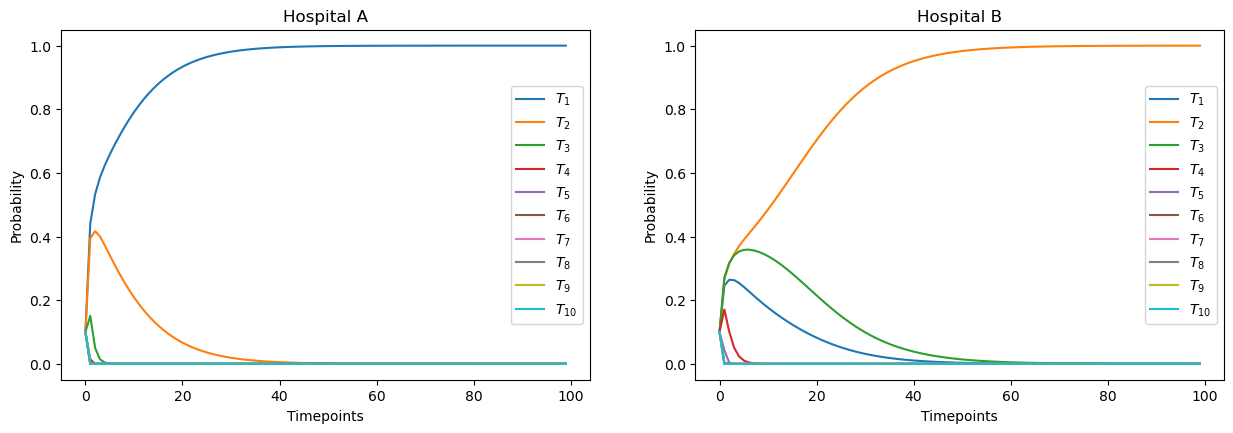
\includegraphics[width=\textwidth]{Bin/replicator_dynamics/ard_t_1.5.png}

        \[T_A = 1  \qquad \qquad \qquad \qquad \qquad \qquad T_B = 2\]
    \end{columns}

\end{frame}


\begin{frame}
    \frametitle{Asymmetric replicator dynamics - \(t = 1.7\)}

    \begin{columns}
        \centering
        \column{\dimexpr\paperwidth-10pt}
        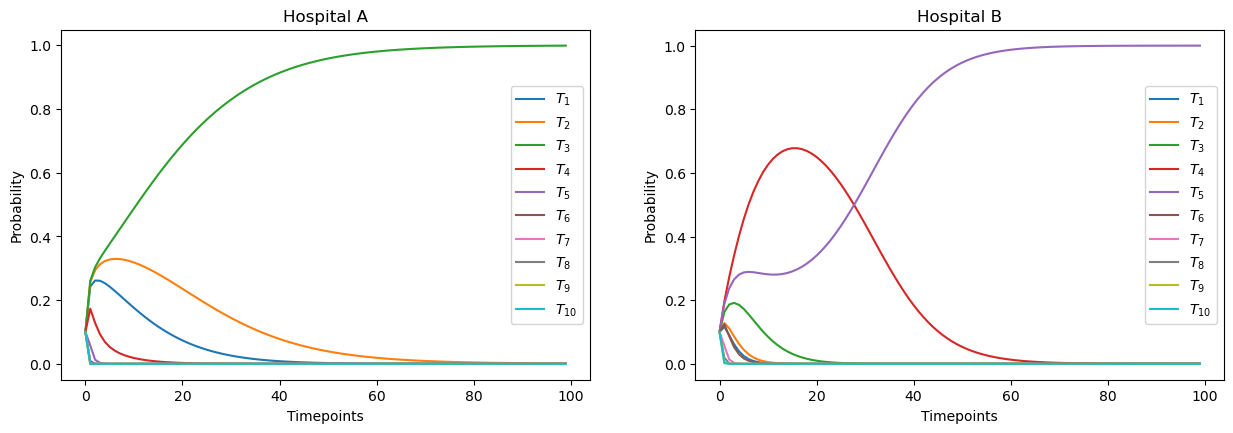
\includegraphics[width=\textwidth]{Bin/replicator_dynamics/ard_t_1.7.png}

        \[T_A = 3  \qquad \qquad \qquad \qquad \qquad \qquad T_B = 5\]
    \end{columns}
    
\end{frame}


\begin{frame}
    \frametitle{Asymmetric replicator dynamics - \(t = 2\)}

    \begin{columns}
        \centering
        \column{\dimexpr\paperwidth-10pt}
        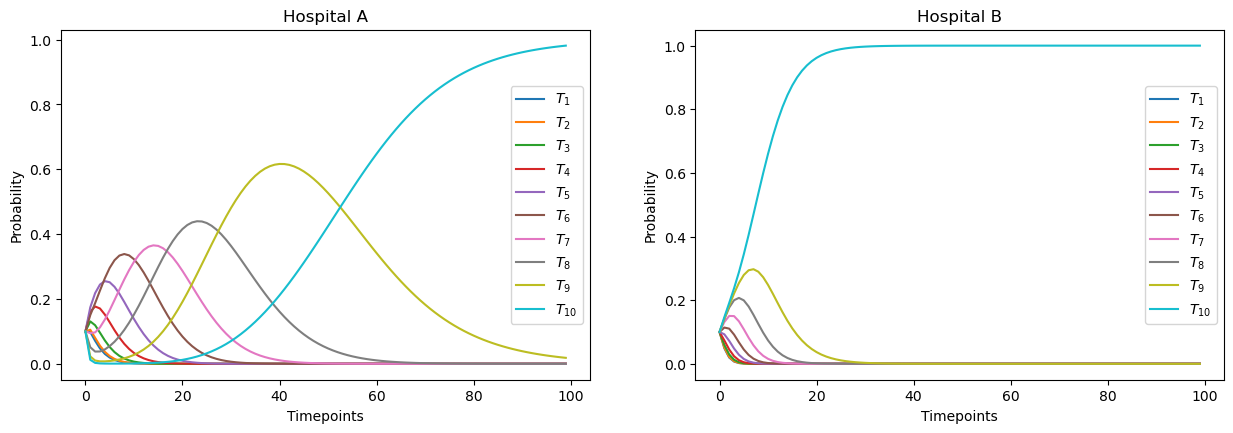
\includegraphics[width=\textwidth]{Bin/replicator_dynamics/ard_t_2.png}

        \[ T_A = 10  \qquad \qquad \qquad \qquad \qquad \qquad T_B = 10\]
    \end{columns}
    
\end{frame}


